\documentclass[11pt]{article}

\usepackage{tikz}
\usepackage{xurl}
\usepackage{float}
\usepackage{amsmath}
\usepackage{booktabs}
\usepackage{graphicx}
\usepackage{listings}
\usepackage[T5]{fontenc}
\usepackage{indentfirst}
\usepackage[utf8]{inputenc}
\usepackage[margin=1in]{geometry}
\usetikzlibrary{arrows.meta, positioning}

\begin{document}

\begin{center}

{\Large \textbf{UNIVERSITY OF SCIENCE AND TECHNOLOGY OF HANOI}}\\
\vspace{0.3cm}
----------------------o0o----------------------\\

\vspace{4cm}

{\large
\centerline{2540027 - Nguyễn Xuân Vinh}
}

\vspace{4cm}

{\Huge \textbf{BC3.04a Advanced Programming for HPC}}\\
\vspace{0.5cm}
Lecturer: Dr. Trần Giang Sơn

\vspace{4cm}

{\Large \textbf{REPORT LABWORK 5}}\\

\vspace{0.5cm}

{\large
Subjects: Gaussian Blur Convolution
}

\vspace{4cm}
\today
\end{center}

\newpage

\newpage

\tableofcontents

\newpage

\section{Introduction}

The labwork 5 will implement a Gaussian blur convolution using CUDA.

The grayscale image from the previous labwork is used as the input.

A $7\times7$ Gaussian filter is applied to the image using two CUDA
implementations. The first implementation accesses the Gaussian filter
from global memory, while the second implementation copies the filter
into shared memory before performing the convolution.

Different two-dimensional CUDA block sizes are also tested to study
their effect on execution time and speedup.

The CPU implementation is used as the baseline for calculating the
GPU speedup.

\section{Image and Grayscale Conversion}

The input image has the following dimensions:

\begin{itemize}
    \item Width: 1080 pixels
    \item Height: 1920 pixels
    \item Channels: 3 (RGB)
    \item Total pixels: 2,073,600
\end{itemize}

The image is converted to grayscale using the weighted RGB formula:

\[
Gray = 0.299R + 0.587G + 0.114B
\]

The resulting grayscale image has dimensions:

\[
1920\times1080
\]

The grayscale image is then used as the input for the Gaussian blur
operation.

\section{7$\times$7 Gaussian Filter}

A two-dimensional Gaussian filter with size $7\times7$ is used.

The Gaussian function is defined as:

\[
G(x,y)=
\frac{1}{2\pi\sigma^2}
e^{-\frac{x^2+y^2}{2\sigma^2}}
\]

In this implementation:

\[
\sigma = 1.0
\]

The filter is generated using NumPy and then normalized so that the sum
of all filter coefficients is equal to 1.

The resulting filter is:

\[
\begin{bmatrix}
1.9652\cdot10^{-5} & 2.3941\cdot10^{-4} & 1.0730\cdot10^{-3} &
1.7690\cdot10^{-3} & 1.0730\cdot10^{-3} & 2.3941\cdot10^{-4} &
1.9652\cdot10^{-5}\\
2.3941\cdot10^{-4} & 2.9166\cdot10^{-3} & 1.3071\cdot10^{-2} &
2.1551\cdot10^{-2} & 1.3071\cdot10^{-2} & 2.9166\cdot10^{-3} &
2.3941\cdot10^{-4}\\
1.0730\cdot10^{-3} & 1.3071\cdot10^{-2} & 5.8582\cdot10^{-2} &
9.6585\cdot10^{-2} & 5.8582\cdot10^{-2} & 1.3071\cdot10^{-2} &
1.0730\cdot10^{-3}\\
1.7690\cdot10^{-3} & 2.1551\cdot10^{-2} & 9.6585\cdot10^{-2} &
1.5924\cdot10^{-1} & 9.6585\cdot10^{-2} & 2.1551\cdot10^{-2} &
1.7690\cdot10^{-3}\\
1.0730\cdot10^{-3} & 1.3071\cdot10^{-2} & 5.8582\cdot10^{-2} &
9.6585\cdot10^{-2} & 5.8582\cdot10^{-2} & 1.3071\cdot10^{-2} &
1.0730\cdot10^{-3}\\
2.3941\cdot10^{-4} & 2.9166\cdot10^{-3} & 1.3071\cdot10^{-2} &
2.1551\cdot10^{-2} & 1.3071\cdot10^{-2} & 2.9166\cdot10^{-3} &
2.3941\cdot10^{-4}\\
1.9652\cdot10^{-5} & 2.3941\cdot10^{-4} & 1.0730\cdot10^{-3} &
1.7690\cdot10^{-3} & 1.0730\cdot10^{-3} & 2.3941\cdot10^{-4} &
1.9652\cdot10^{-5}
\end{bmatrix}
\]

The measured sum of the filter coefficients is:

\[
\boxed{1.0}
\]

Therefore, the filter preserves the overall average intensity while
performing the smoothing operation.

\section{CPU Gaussian Blur}

The CPU implementation performs the same $7\times7$ convolution as the
CUDA implementations.

Zero padding is used at the image boundaries. For each output pixel,
the implementation multiplies the $7\times7$ neighborhood by the
corresponding Gaussian filter coefficients and sums the results.

The measured CPU execution time was:

\[
\boxed{T_{CPU}=48.151962\text{ s}}
\]

This execution time is used as the baseline for calculating the GPU
speedup.

The CPU result is also used to validate the CUDA results.

\section{CUDA Implementation Without Shared Memory}

The first CUDA implementation performs the Gaussian convolution using
global memory.

Each CUDA thread calculates one output pixel.

The two-dimensional CUDA grid is obtained using:

\begin{verbatim}
x, y = cuda.grid(2)
\end{verbatim}

For each output pixel, the kernel processes all 49 values of the
$7\times7$ Gaussian filter.

The filter is accessed directly from global memory:

\begin{verbatim}
value += image[iy, ix] * kernel[ky, kx]
\end{verbatim}

Zero padding is implemented by checking whether the calculated input
coordinates are inside the image boundaries.

The execution time is measured using \texttt{time.time()} and
\texttt{cuda.synchronize()} is used before recording the end time.

\section{CUDA Implementation With Shared Memory}

The second implementation uses shared memory for the Gaussian filter.

A shared-memory array of size $7\times7$ is allocated:

\begin{verbatim}
shared_kernel = cuda.shared.array(
    (7, 7), dtype=np.float32
)
\end{verbatim}

The 49 filter values are copied cooperatively by the threads in each
block.

Because a $4\times4$ block contains only 16 threads, each thread may
copy more than one filter value. The implementation therefore uses a
loop to ensure that all 49 values are copied:

\begin{verbatim}
for i in range(tid, 49, threads):
    ky = i // 7
    kx = i % 7
    shared_kernel[ky, kx] = kernel[ky, kx]
\end{verbatim}

A synchronization barrier is then used:

\begin{verbatim}
cuda.syncthreads()
\end{verbatim}

This ensures that all filter values have been copied before the
convolution begins.

The convolution then uses \texttt{shared\_kernel} instead of directly
accessing the filter in global memory.

The image itself is not copied into shared memory. Only the $7\times7$
Gaussian filter is stored in shared memory.

\section{Block Size Experiment}

Six different two-dimensional block configurations were tested:

\[
4\times4,\quad
8\times8,\quad
16\times16,\quad
32\times8,\quad
8\times32,\quad
32\times16
\]

Each configuration was measured five times and the average GPU execution
time was used.

The speedup is calculated using:

\[
Speedup =
\frac{T_{CPU}}{T_{GPU}}
\]

The measured results are shown in Table~\ref{tab:block-results}.

\begin{table}[H]
    \centering
    \caption{Gaussian blur performance for different 2D block sizes}
    \label{tab:block-results}
    \begin{tabular}{c c c c c}
        \toprule
        Block Size &
        Threads/Block &
        Global Time (s) &
        Global Speedup &
        Shared Time (s) /
        Shared Speedup \\
        \midrule
        $4\times4$ &
        16 &
        0.010148 &
        4745.10$\times$ &
        0.010145 / 4746.58$\times$ \\

        $8\times8$ &
        64 &
        0.005110 &
        9423.83$\times$ &
        0.005102 / 9438.72$\times$ \\

        $16\times16$ &
        256 &
        0.003264 &
        14753.96$\times$ &
        0.002731 / 17630.46$\times$ \\

        $32\times8$ &
        256 &
        0.002699 &
        17842.92$\times$ &
        0.002801 / 17192.81$\times$ \\

        $8\times32$ &
        256 &
        0.002709 &
        17774.76$\times$ &
        0.002689 / 17906.83$\times$ \\

        $32\times16$ &
        512 &
        0.002696 &
        17860.27$\times$ &
        0.002681 / 17961.29$\times$ \\

        \bottomrule
    \end{tabular}
\end{table}

The results show that the block size has a significant effect on GPU
execution time.

The $4\times4$ configuration has only 16 threads per block and has the
highest execution time among the tested configurations.

Larger configurations generally provide better performance in this
experiment. The best measured configurations for both implementations
were $32\times16$.

\section{Speedup Graph}

The relationship between block size and speedup is shown in
Figure~\ref{fig:speedup}.

\begin{figure}[H]
    \centering
    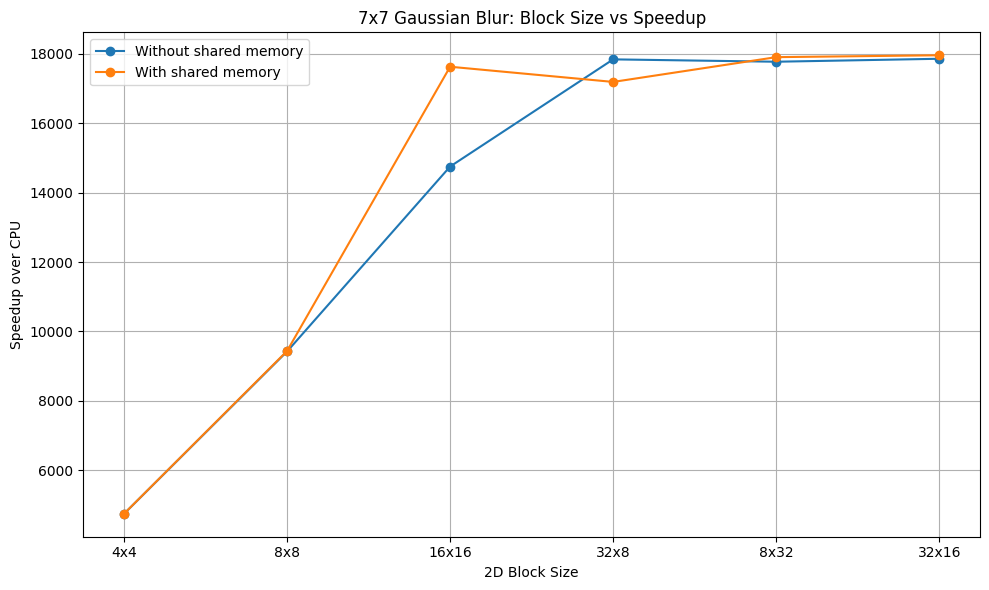
\includegraphics[width=0.85\textwidth]
    {gaussian_block_size_vs_speedup.png}
    \caption{2D block size versus Gaussian blur speedup}
    \label{fig:speedup}
\end{figure}

The graph compares the global-memory and shared-memory implementations
for all tested block sizes.

The largest measured speedup for the global-memory implementation was:

\[
\boxed{17860.27\times}
\]

using a $32\times16$ block.

The largest measured speedup for the shared-memory implementation was:

\[
\boxed{17961.29\times}
\]

also using a $32\times16$ block.

\section{Execution Time Graph}

The GPU execution times for the tested block sizes are shown in
Figure~\ref{fig:execution-time}.

\begin{figure}[H]
    \centering
    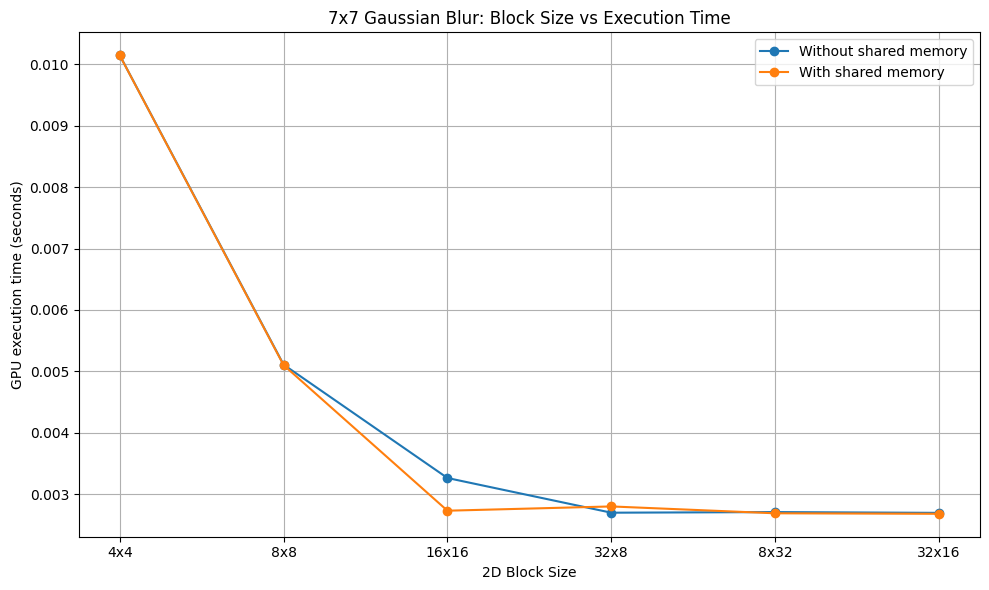
\includegraphics[width=0.85\textwidth]
    {gaussian_block_size_vs_time.png}
    \caption{2D block size versus GPU execution time}
    \label{fig:execution-time}
\end{figure}

The results show that the best measured global-memory execution time was:

\[
\boxed{0.002696\text{ s}}
\]

while the best measured shared-memory execution time was:

\[
\boxed{0.002681\text{ s}}
\]

Both were obtained using the $32\times16$ block configuration.

\section{Best Configuration Comparison}

The best configurations are summarized in Table~\ref{tab:best}.

\begin{table}[H]
    \centering
    \caption{Best measured GPU configurations}
    \label{tab:best}
    \begin{tabular}{lccc}
        \toprule
        Implementation &
        Block Size &
        GPU Time (s) &
        Speedup \\
        \midrule
        Global memory &
        $32\times16$ &
        0.002696 &
        17860.27$\times$ \\

        Shared memory &
        $32\times16$ &
        0.002681 &
        17961.29$\times$ \\

        \bottomrule
    \end{tabular}
\end{table}

The ratio between the best global-memory and shared-memory execution
times is:

\[
\frac{0.002696}{0.002681}
\approx 1.01
\]

Thus, in this experiment, the shared-memory implementation was measured
at approximately $1.01\times$ the performance of the global-memory
implementation.

The difference is small. This is reasonable because only the $7\times7$
filter is stored in shared memory, while the image data remains in
global memory.

\section{Validation}

The CUDA results were compared with the CPU Gaussian blur result.

For the global-memory implementation, the measured differences were:

\[
\text{Maximum difference}
=
0.0001373291
\]

\[
\text{Mean difference}
=
8.7052285\times10^{-6}
\]

For the shared-memory implementation, the measured differences were
the same:

\[
\text{Maximum difference}
=
0.0001373291
\]

\[
\text{Mean difference}
=
8.7052285\times10^{-6}
\]

Both implementations passed the numerical validation using
\texttt{np.allclose()}.

Therefore:

\[
\boxed{\text{Global-memory validation: PASS}}
\]

\[
\boxed{\text{Shared-memory validation: PASS}}
\]

The results confirm that the two CUDA implementations produce the same
Gaussian-blurred image as the CPU implementation within floating-point
tolerance.

\section{Discussion}

The experiment demonstrates that the CUDA block configuration has a
significant effect on the execution time of the Gaussian blur operation.

The $4\times4$ block uses only 16 threads and produced an execution time
of approximately $0.010$ seconds for both implementations.

Increasing the block size improved the measured performance. For example,
the $32\times16$ configuration used 512 threads per block and produced
the lowest measured execution time for both implementations.

The best global-memory result was:

\[
0.002696\text{ s}
\]

with a speedup of:

\[
17860.27\times
\]

The best shared-memory result was:

\[
0.002681\text{ s}
\]

with a speedup of:

\[
17961.29\times
\]

Although shared memory was slightly faster in the final measurement,
the difference was small, with a measured ratio of approximately
$1.01\times$.

This experiment only places the Gaussian filter in shared memory. The
image pixels are still accessed from global memory. Therefore, the
shared-memory implementation does not eliminate global-memory accesses
for the image itself.

The reported GPU times measure the CUDA kernel execution and synchronization
after the input data has already been transferred to the GPU. Therefore,
the reported speedups do not represent the complete image-processing
pipeline including host-to-device and device-to-host memory transfers.

\section{Conclusion}

Labwork 5 successfully implemented a $7\times7$ Gaussian blur
convolution using CUDA.

Two CUDA implementations were developed. The first accesses the Gaussian
filter from global memory, while the second copies the filter into shared
memory before performing the convolution.

Six different 2D block sizes were tested to study their effect on
performance.

The best measured global-memory configuration was $32\times16$, with an
execution time of:

\[
\boxed{0.002696\text{ s}}
\]

and a speedup of:

\[
\boxed{17860.27\times}
\]

The best measured shared-memory configuration was also $32\times16$,
with an execution time of:

\[
\boxed{0.002681\text{ s}}
\]

and a speedup of:

\[
\boxed{17961.29\times}
\]

The shared-memory implementation achieved a measured performance ratio
of approximately $1.01\times$ compared with the global-memory version.

Finally, both CUDA implementations passed numerical validation, with a
maximum difference of $0.0001373291$ and a mean difference of
$8.7052285\times10^{-6}$ compared with the CPU result.

Therefore, the implementation satisfies the requirements of the
Gaussian blur convolution labwork and demonstrates the effect of CUDA
2D block size and shared memory on GPU performance.

\end{document}